\documentclass[manuscript,review]{acmart}

\usepackage{booktabs}
\usepackage{amsmath}
\usepackage{graphicx}
\usepackage{algorithm}
\usepackage{algpseudocode}

\title{Enabling Auto-Correction on Soft Braille Keyboard}

\author{Dan Zhang}
\affiliation{%
  \institution{Computer Science Department, Stony Brook University}
  \city{Stony Brook}
  \state{New York}
  \country{USA}
}
\email{zhang64@cs.stonybrook.edu}

\author{Yan Ma}
\affiliation{%
  \institution{Computer Science Department, Stony Brook University}
  \city{Stony Brook}
  \state{New York}
  \country{USA}
}
\email{yanma1@cs.stonybrook.edu}

\author{Glenn Dausch}
\affiliation{%
  \institution{Computer Science Department, Stony Brook University}
  \city{Stony Brook}
  \state{New York}
  \country{USA}
}
\email{glenn.dausch@stonybrook.edu}

\author{William H Seiple}
\affiliation{%
  \institution{Lighthouse Guild}
  \city{New York}
  \state{New York}
  \country{USA}
}
\email{wseiple@lighthouseguild.org}

\author{David Xianfeng Gu}
\affiliation{%
  \institution{Department of Computer Science, Stony Brook University}
  \city{Stony Brook}
  \state{New York}
  \country{USA}
}
\email{gu@cs.stonybrook.edu}

\author{IV Ramakrishnan}
\affiliation{%
  \institution{Computer Science Department, Stony Brook University}
  \city{Stony Brook}
  \state{New York}
  \country{USA}
}
\email{ram@cs.stonybrook.edu}

\author{Xiaojun Bi}
\affiliation{%
  \institution{Department of Computer Science, Stony Brook University}
  \city{Stony Brook}
  \state{New York}
  \country{USA}
}
\email{xiaojun@cs.stonybrook.edu}

\begin{document}

\begin{abstract}
A soft Braille keyboard is a graphical representation of the Braille writing system on smartphones. It provides an essential text input method for visually impaired individuals, but accuracy and efficiency remain significant challenges. We present an intelligent Braille keyboard with auto-correction ability, which uses optimal transportation theory to estimate the distances between touch input and Braille patterns, and combines it with a language model to estimate the probability of entering words. The proposed system was evaluated through both simulations and user studies. In a touch interaction simulation on an Android phone and an iPhone, our intelligent Braille keyboard demonstrated superior error correction performance compared to the Android Braille keyboard with proofreading suggestions and the iPhone Braille keyboard with spelling suggestions. It reduced the error rate from 55.81\% on Android and 57.13\% on iPhone to 19.80\% under high typing noise. Furthermore, in a user study of 12 participants who are legally blind, the intelligent Braille keyboard reduced word error rate (WER) by 59.5\% (42.53\% to 17.28\%) with a slight drop of 0.74 words per minute (WPM), compared to a conventional Braille keyboard without auto-correction. These findings suggest that our approach has the potential to greatly improve the typing experience for Braille users on touchscreen devices.
\end{abstract}

\maketitle

\section{Introduction}

Smartphones have become indispensable tools for modern life, yet they present significant accessibility barriers for people who are blind or visually impaired. Text entry, a fundamental interaction method for activities ranging from messaging to web browsing, remains particularly challenging. Standard QWERTY soft keyboards are inefficient for blind users, often yielding low typing speeds of around 5 words per minute (WPM) and high error rates \cite{Billah2019, Southern2012, Nicolau2015}. While voice input offers speed, it poses privacy concerns and makes error correction difficult \cite{Hong2020}.

Soft Braille keyboards, which replicate the six-dot Braille layout on touchscreens, offer a promising alternative. However, current implementations on major mobile operating systems deterministically map touch inputs to Braille dots. This lack of intelligence means that even slight deviations in finger placement result in errors. Research has shown that error rates on these keyboards can exceed 40\% for some user groups \cite{Frey2011}.

While auto-correction via statistical decoding has revolutionized QWERTY typing for sighted users \cite{Goodman2002}, these techniques are not directly transferable to Braille. Standard decoders assume a single touch point per character mapped via a Gaussian distribution \cite{Bi2016}. In contrast, Braille characters are formed by simultaneous multi-touch patterns (chords) where the number of touch points may not even match the target character's dot count due to input errors.

To address this gap, we propose an intelligent Braille keyboard powered by Optimal Transport (OT) theory \cite{Villani2009}. This mathematical framework calculates the minimal cost to transform the user's touch distribution into the standard Braille dot pattern distribution. By integrating this spatial model with a language model, our system can infer the intended word even amidst significant input noise.

\begin{figure}[h]
  \centering
  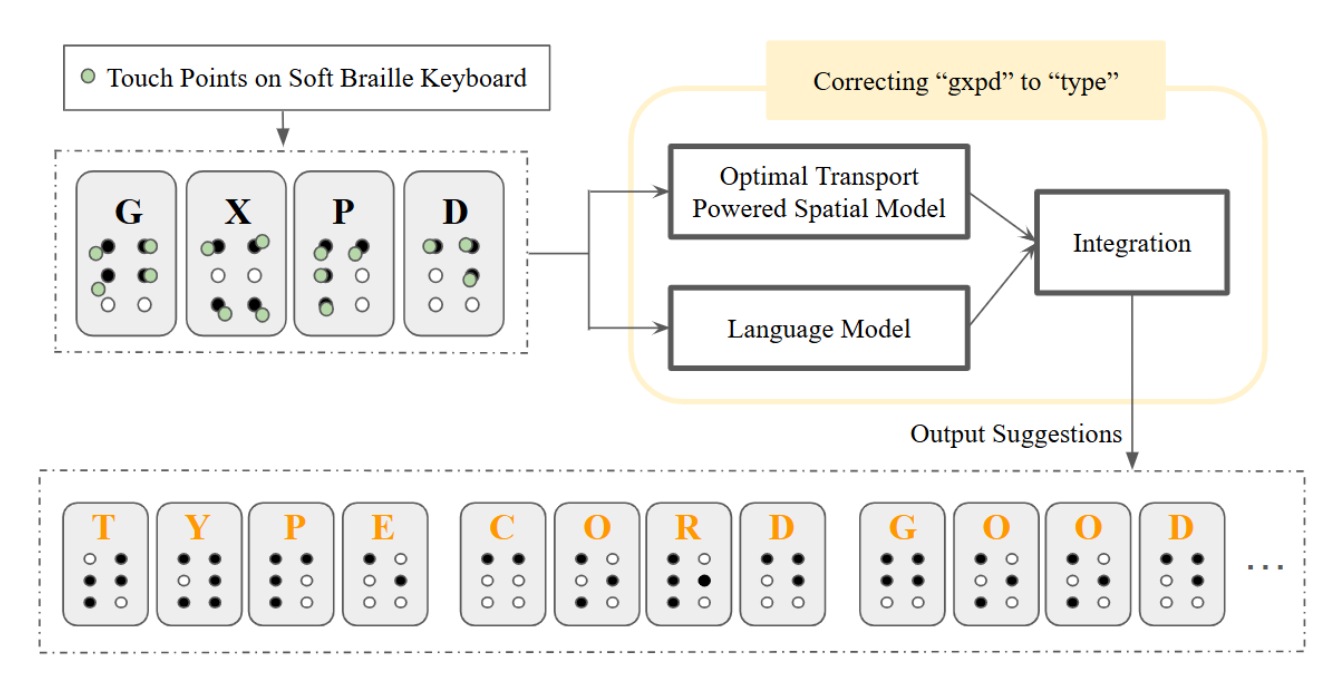
\includegraphics[width=\textwidth]{Figure 1.png}
  \caption{Illustration of word auto-correction on the proposed intelligent Braille keyboard. In this example, the user wants to type word ``type'', but mistakenly has a dispositional touch for letter ‘t’, an omitted touch for letter ‘y’, and an extra touch for letter ‘e’. The touch input positions are initially mapped to letters: ‘g’, ‘x’, ‘p’, and ‘d’. The keyboard then utilizes two modules—spacial model powered by optimal transport and a language model—to compute the likelihood of each candidate word being the intended word. After integrating these probabilities, the keyboard displays the top three candidate words with the highest probabilities at the bottom: “type”, “cord”, and “good”.}
  \label{fig:1}
\end{figure}

\section{Background and Related Work}

\subsection{Text Entry Techniques for Visually Impaired Individuals}
The primary method for text entry among blind users is the ''explore by touch'' method on QWERTY keyboards, which is notoriously slow. Studies indicate average speeds of approximately 5 WPM, drastically slower than the 36 WPM average for sighted users \cite{Palin2019}. While voice input is an alternative, correcting recognition errors is a tedious process requiring precise cursor manipulation, often consuming up to 80\% of the interaction time \cite{Azenkot2013}.

Soft Braille keyboards utilize the screen to represent the Perkins Brailler layout. While they theoretically allow for faster entry, the lack of tactile feedback on glass surfaces leads to high error rates due to finger drift and imprecise targeting \cite{Oliveira2011}.

\subsection{Statistical Decoding}
In the domain of virtual keyboards, statistical decoding is the standard for error correction. It treats touch points as signals distributed spatially. Using Bayes' rule, the probability of a word is calculated by combining the spatial probability of the touch points with the prior probability from a language model \cite{Goodman2002}. While advanced models like the Dual Gaussian distribution \cite{Bi2016} handle finger variability well, they are designed for single-finger tapping sequences, not the multi-touch chording inherent to Braille.

\subsection{On-screen Braille Keyboards}
Various designs have been explored, such as BrailleTouch \cite{Frey2011} and TypeInBraille \cite{Mascetti2011}. Commercial implementations exist in iOS and Android (TalkBack). However, error correction in these systems is generally limited to basic spell-checking after the fact, rather than correcting the touch input itself. Exceptions like B\# \cite{Nicolau2014} use chord-based correction but do not utilize the robust spatial mapping offered by Optimal Transport.

\begin{figure}[h]
  \centering
  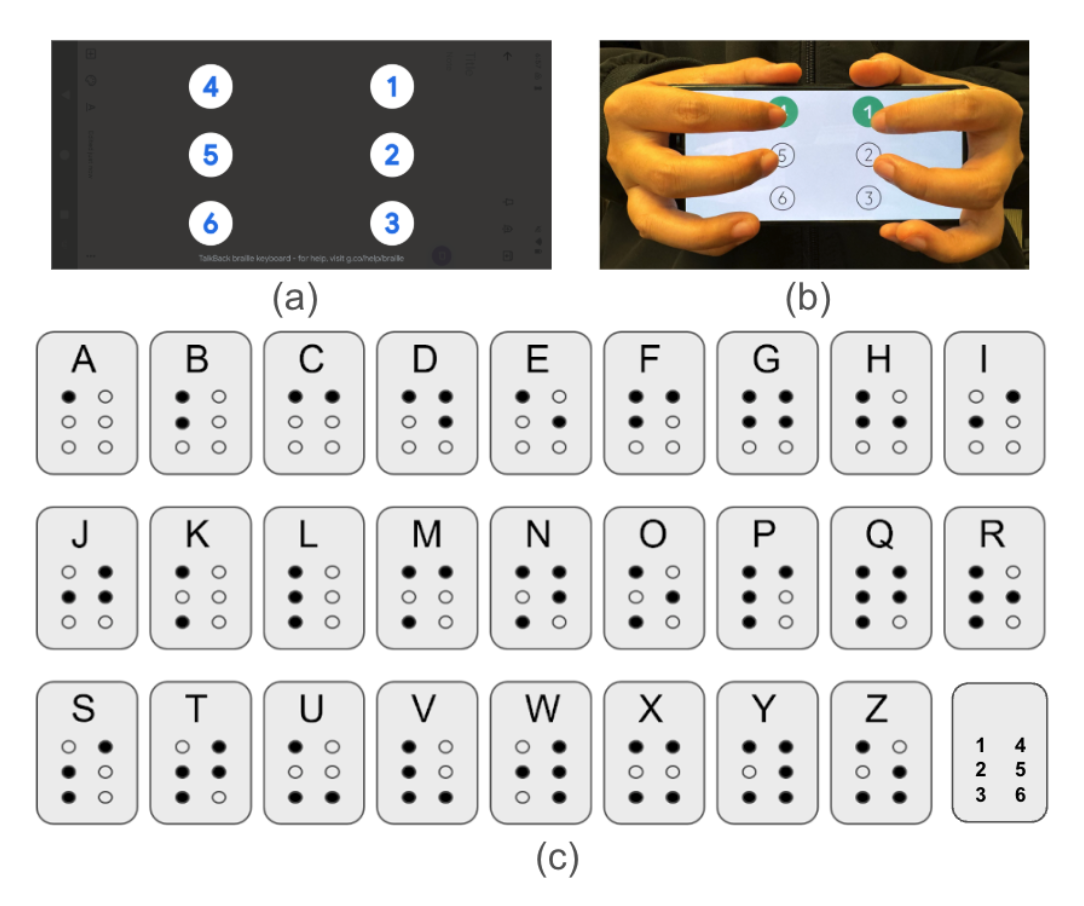
\includegraphics[width=\textwidth]{Figure 2.png}
  \caption{(a) Screenshot of an existing conventional Braille keyboard. (b) Entering ‘c’ on the intelligent Braille keyboard. (c) Mappings between Braille input and letters, and the numbering of Braille dots. Note that the numbering of Braille dots on the touchscreen mirrors the layout in (c), as the touchscreen is facing away during typing.}
  \label{fig:2}
\end{figure}

\section{Method: Intelligent Braille Keyboard}

Our system improves upon standard Braille keyboards by introducing a decoding algorithm that handles the ambiguity of touch inputs.

\subsection{Decoding Principle}
The decoding process parallels QWERTY statistical decoders but employs a novel spatial model. We compute the posterior probability of a word candidates using two components:
\begin{enumerate}
    \item A Spatial Model: Infers the probability of a character based on touch locations.
    \item A Language Model: Infers the probability based on linguistic context.
\end{enumerate}

\subsection{Representing Inputs as Distributions}
The core innovation is representing both the user's input and the target Braille characters as discrete mass distributions.
\begin{itemize}
    \item \textbf{User Input ($p$):} If a user touches the screen with $m$ fingers, we treat this as a distribution of mass 1, evenly divided among the $m$ points ($1/m$ mass at each location).
    \item \textbf{Braille Pattern ($c$):} A Braille character with $n$ dots is represented as mass 1 evenly distributed among the $n$ standard dot locations ($1/n$ mass each).
\end{itemize}

This formulation allows us to compare inputs where the number of touches does not match the number of required dots (e.g., touching 4 points for a 2-dot letter).

\begin{figure}[h]
  \centering
  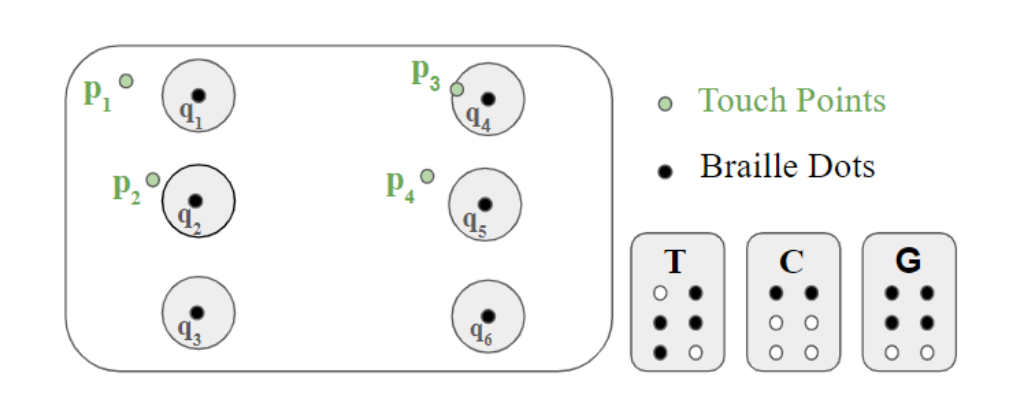
\includegraphics[width=0.6\textwidth]{Figure 3.png}
  \caption{Illustration of Braille input and the Braille dot patterns of three candidate characters, ‘t’, ‘c’ and ‘g’, for the example in Section 3.2 and 3.3.}
  \label{fig:3}
\end{figure}

\subsection{Squared Wasserstein-2 Distance}
To quantify the difference between the user's input $p$ and a target character $c$, we utilize the Optimal Transport theory, specifically the squared Wasserstein-2 distance ($W_2^2$). This metric effectively measures the "effort" to move the mass from the touch points to the Braille dot locations.

First, a cost matrix $M$ is generated, where $M_{ij}$ is the squared Euclidean distance between a touch point $p_i$ and a Braille dot location $q_j$:
\begin{equation}
    M_{ij} = ||p_i - q_j||^2
\end{equation}

The distance is then found by minimizing the transportation cost:
\begin{equation}
    W_2^2(p, c) = \min_{Y \in T} \sum_{i=1}^m \sum_{j=1}^6 M_{ij} Y_{ij}
\end{equation}
where $Y$ represents the transportation plan. We solve this using the network simplex method via the POT package \cite{Flamary2021}.

\subsection{Spatial and Language Scoring}
The calculated transport cost is converted into a spatial probability using a Gaussian function:
\begin{equation}
    P(c|p) = \frac{1}{\sqrt{2\pi\sigma^2}} \exp\left(-\frac{W_2^2(p,c)}{2\sigma^2}\right)
\end{equation}

Finally, this spatial score is combined with a bigram language model score $L(w)$ (trained on the COCA corpus) to determine the final candidate score.

\section{Comparison with Android and iPhone Keyboards}

To validate our approach, we conducted extensive simulations comparing our Intelligent Braille Keyboard against the native correction features of Android (TalkBack proofread) and iOS (VoiceOver spellcheck).

\subsection{Simulation Setup}
We utilized automation tools (AutoTouch for iOS, Appium for Android) to simulate typing on physical devices (iPhone 6s and Google Pixel 6). The test set consisted of 200 sentences from a standard text entry dataset \cite{Vertanen2011}.

\subsection{Simulation I: Statistical Noise}
We introduced Gaussian noise to the touch coordinates to simulate imprecise typing. We tested at two noise levels: High ($SD=7.8$ mm) and Low ($SD=3.9$ mm). As shown in Table 1, our system significantly outperformed both competitors. Under high noise, our Top-1 Error Rate was only 19.80\%, compared to over 55\% for both Android and iPhone.

\begin{table}[h]
  \caption{Simulation I results: WER (\%) with Gaussian noise on Android Braille keyboard, iPhone Braille keyboard, and our intelligent Braille keyboard with auto-correction}
  \label{tab:sim1}
  \begin{tabular}{lcccc}
    \toprule
    Braille Keyboards & \multicolumn{2}{c}{SD = 7.8 mm} & \multicolumn{2}{c}{SD = 3.9 mm} \\
    \cmidrule(lr){2-3} \cmidrule(lr){4-5}
    & Top-1 & Top-3 & Top-1 & Top-3 \\
    \midrule
    Android & 55.81 & 52.74 & 7.49 & 6.82 \\
    iPhone & 57.13 & 52.82 & 8.63 & 7.96 \\
    Auto-correction & 19.80 & 12.29 & 1.30 & 0.00 \\
    \bottomrule
  \end{tabular}
\end{table}

\subsection{Simulation II: Specific Typing Errors}
We also simulated specific error types common in Braille typing:
\begin{itemize}
    \item \textbf{Disposition:} Touching the wrong dots.
    \item \textbf{Omission:} Missing a required dot.
    \item \textbf{Extra:} Adding an unintended dot.
\end{itemize}

Table 2 highlights the robustness of our OT-based decoder. While existing keyboards struggled significantly (WER > 45\%), our system maintained low error rates, particularly for omitted and extra dots.

\begin{table}[h]
  \caption{Simulation II results: WER (\%) for handling different typing errors on Android Braille keyboard, iPhone Braille keyboard, and our intelligent Braille keyboard}
  \label{tab:sim2}
  \begin{tabular}{lccc}
    \toprule
    Braille Keyboards & Disposition & Omitted & Extra \\
    & Top-1/Top-3 & Top-1/Top-3 & Top-1/Top-3 \\
    \midrule
    Android & 64.79 / 60.02 & 64.41 / 60.50 & 59.06 / 54.58 \\
    iPhone & 55.29 / 46.46 & 48.58 / 37.85 & 47.36 / 34.39 \\
    Auto-correction & 19.54 / 10.49 & 11.49 / 6.90 & 14.02 / 8.04 \\
    \bottomrule
  \end{tabular}
\end{table}

\begin{figure}[h]
  \centering
  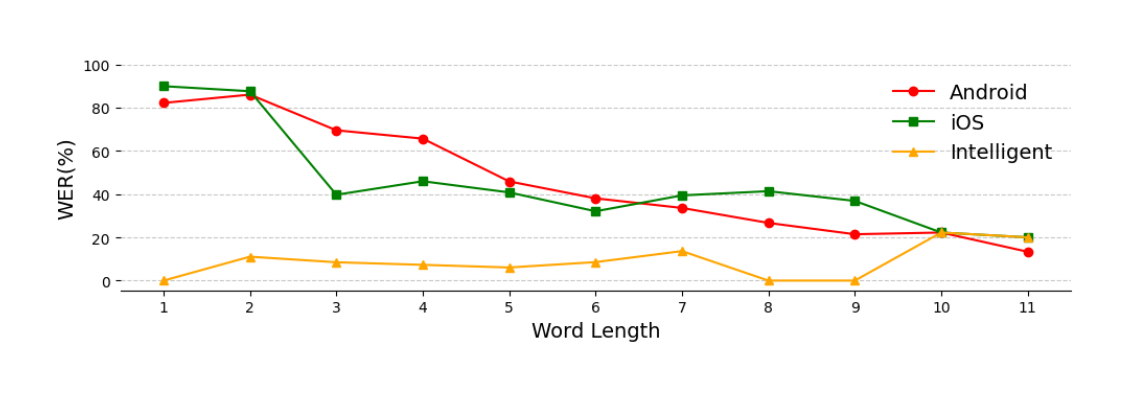
\includegraphics[width=\textwidth]{Figure 4.png}
  \caption{WER on Top-3 Suggestions Across Different Word Lengths}
  \label{fig:4}
\end{figure}

\subsection{Simulation III: Multi-letter Errors}
We further tested the system's ability to correct words containing errors in two separate letters. As shown in Table 3, the system remained effective, though disposition errors remained the most challenging to correct.

\begin{table}[h]
  \caption{Simulation III results: WER (\%) results with two letters mistyped in a word on our Intelligent Braille keyboard}
  \label{tab:sim3}
  \begin{tabular}{lccc}
    \toprule
    & Disposition & Omitted & Extra \\
    \midrule
    Top-1 & 34.79 & 19.08 & 17.93 \\
    Top-3 & 20.96 & 8.59 & 5.06 \\
    \bottomrule
  \end{tabular}
\end{table}

\section{Findings and Results: User Evaluation}

To assess real-world performance, we conducted a user study with 12 legally blind participants (6 men, 6 women, average age 49.3).

\subsection{Apparatus and Procedure}
We implemented the Intelligent Braille Keyboard as a web-based prototype running on a Google Pixel 6. Participants held the device in "screen-away" mode (fingers curling back to touch the screen), as depicted in Figure 5. The task involved transcribing phrases selected from the T-40 dataset.

\begin{figure}[h]
  \centering
  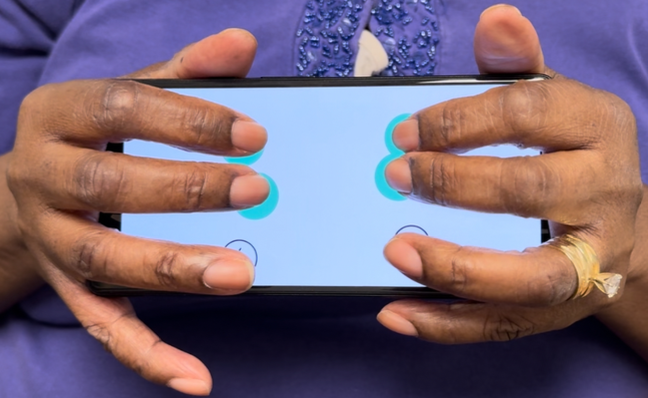
\includegraphics[width=\textwidth]{Figure 5.png}
  \caption{A user is typing letter "g" in screen-away mode on the intelligent Braille keyboard}
  \label{fig:5}
\end{figure}

\begin{figure}[h]
  \centering
  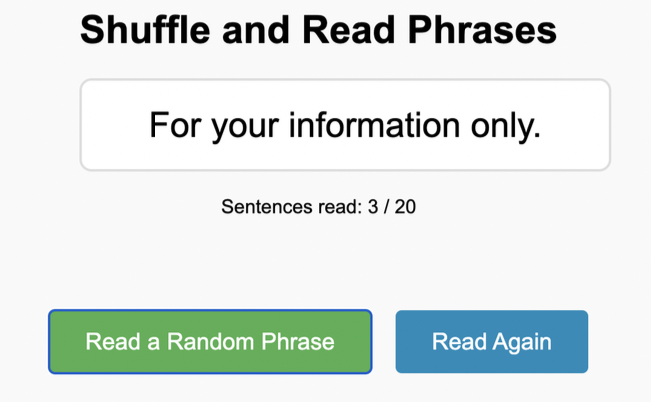
\includegraphics[width=0.8\textwidth]{Figure 6.png}
  \caption{A webpage screenshot of our transcription task}
  \label{fig:6}
\end{figure}

\subsection{Input Speed and Error Rate}
The study compared the intelligent keyboard against the standard TalkBack Braille keyboard.
\begin{itemize}
    \item \textbf{Word Error Rate (WER):} The intelligent keyboard dramatically reduced errors. The average WER dropped from 42.53\% (Conventional) to 17.28\% (Intelligent). This represents a 59.5\% improvement.
    \item \textbf{Typing Speed (WPM):} There was a slight reduction in speed (6.18 WPM Conventional vs. 5.44 WPM Intelligent). This was attributed to the time required for users to navigate the suggestion lists provided by the auto-correction system.
\end{itemize}

Figure 7 illustrates the individual WER improvements, showing that almost every participant benefited from the auto-correction.

\begin{figure}[h]
  \centering
  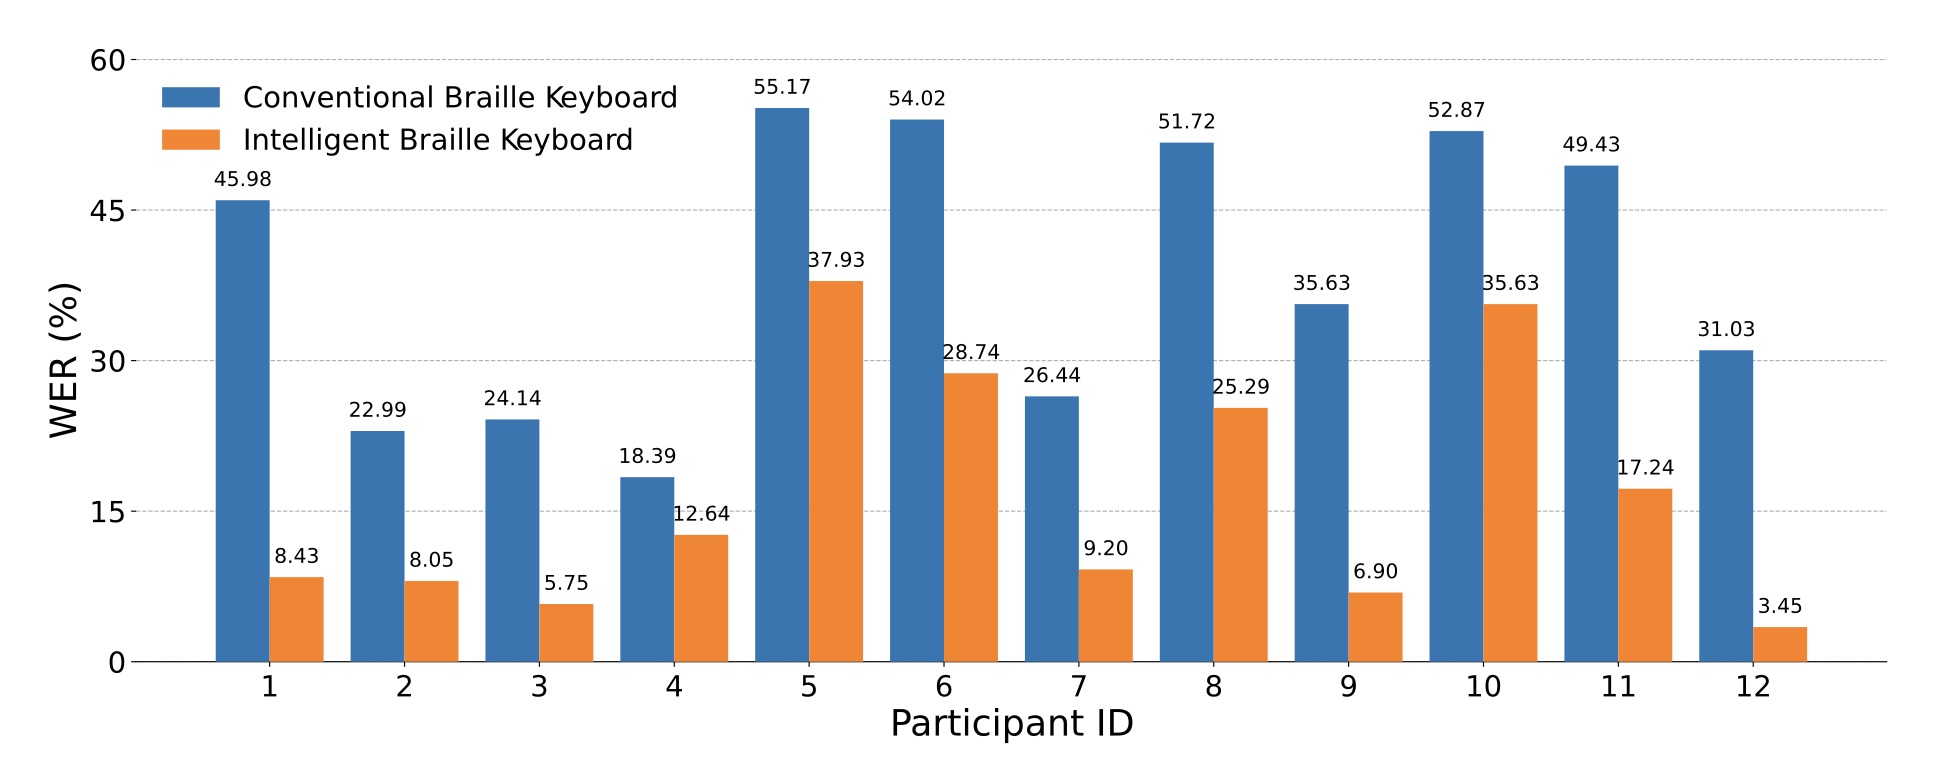
\includegraphics[width=\textwidth]{Figure 7.png}
  \caption{Average WER for the 12 participants}
  \label{fig:7}
\end{figure}

\subsection{Learning Effect}
We analyzed performance across four blocks of trials (Figure 8). While the intelligent keyboard initially had higher error rates as users adapted to the system, the accuracy improved significantly by Block 3. By Block 4, users achieved speeds of 6.81 WPM, nearing the conventional keyboard's speed, but with much higher accuracy.

\begin{figure}[h]
  \centering
  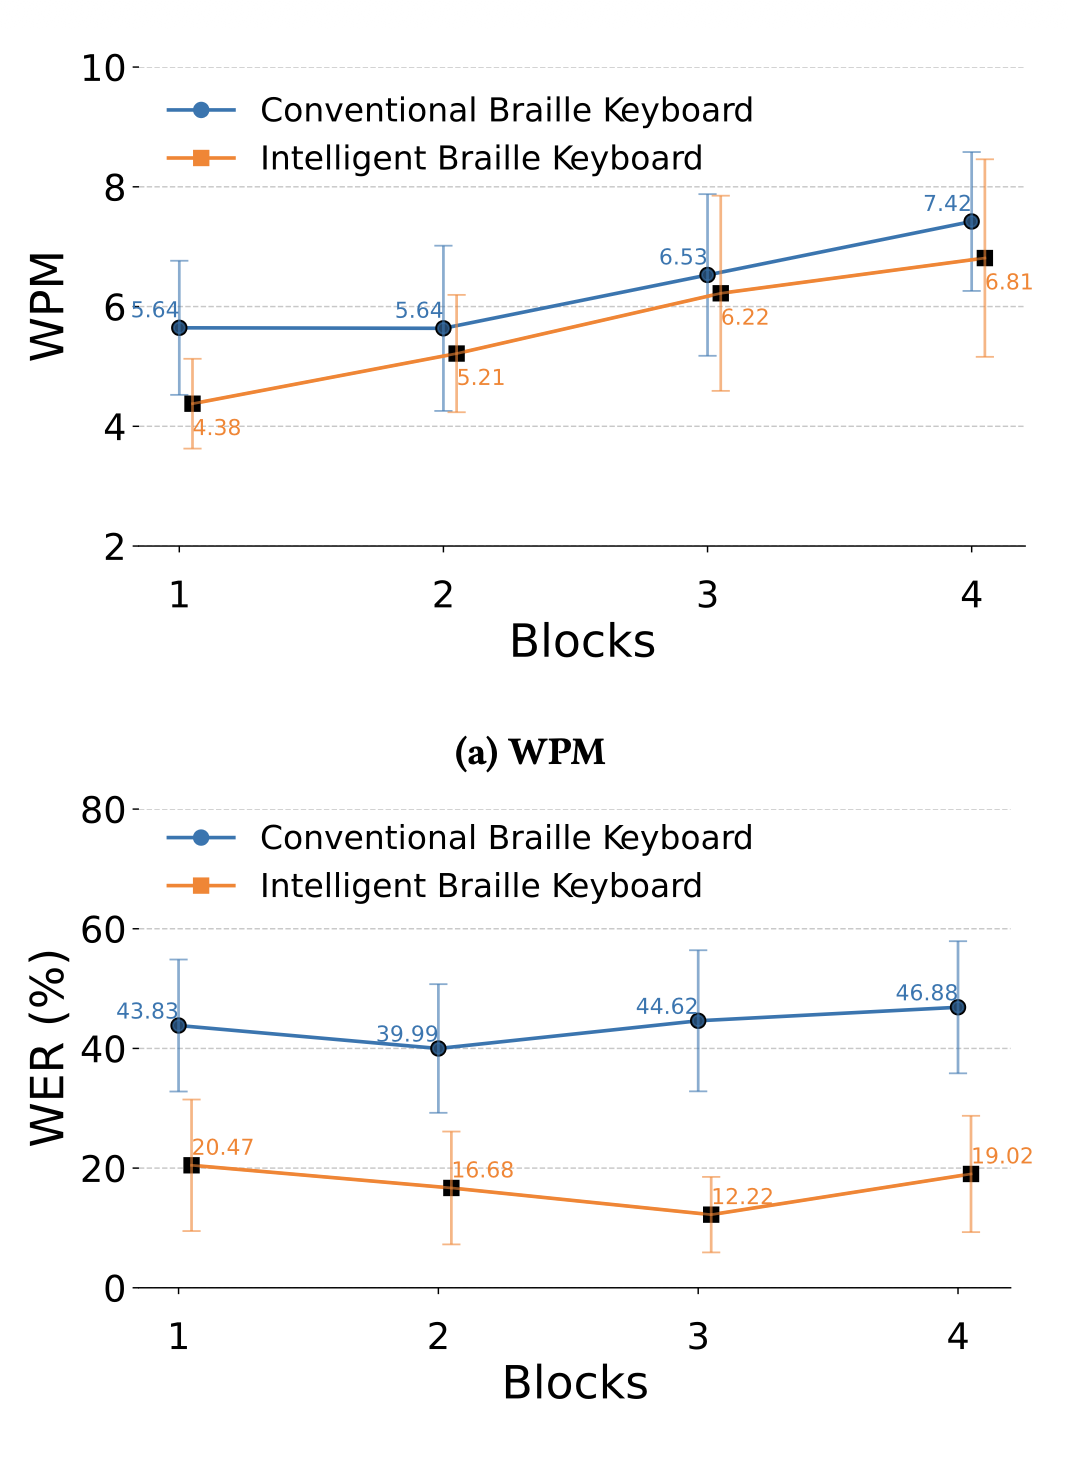
\includegraphics[width=0.8\textwidth]{Figure 8.png}
  \caption{Average(95\%CI) of WPM and WER(\%) by block}
  \label{fig:8}
\end{figure}

\subsection{Suggestion Usage}
Table 4 details how participants utilized the suggestion feature (activated by swiping up). The high accuracy rate of accepted suggestions (mean 74.5\%) validates the effectiveness of the language and spatial model integration.

\begin{table}[h]
  \caption{Analysis of Suggestion Usage: Frequency of Swipe-Up Gestures and Correct Suggestions Adopted}
  \label{tab:sugg}
  \resizebox{\textwidth}{!}{%
  \begin{tabular}{lccccccccccccc}
    \toprule
    & P1 & P2 & P3 & P4 & P5 & P6 & P7 & P8 & P9 & P10 & P11 & P12 & Mean \\
    \midrule
    Suggestion Usage & 17 & 14 & 15 & 24 & 36 & 25 & 16 & 30 & 13 & 45 & 25 & 19 & 23.3 \\
    Correct Suggestion & 15 & 10 & 12 & 17 & 25 & 15 & 15 & 24 & 9 & 29 & 17 & 15 & 16.9 \\
    Accuracy Rate (\%) & 88.2 & 71.4 & 80.0 & 70.8 & 69.4 & 60.0 & 93.8 & 80.0 & 69.2 & 64.4 & 68.0 & 78.9 & 74.5 \\
    \bottomrule
  \end{tabular}%
  }
\end{table}

\subsection{Usability}
Participants rated the systems using the System Usability Scale (SUS) \cite{Brooke1996}. The Intelligent Braille Keyboard received a significantly higher median score of 81.5 compared to 71.25 for the conventional keyboard, indicating higher user satisfaction despite the slight speed trade-off.

\section{Discussion}

The results from both the simulation and the user study provide compelling evidence that integrating Optimal Transport-based decoding into Braille keyboards significantly enhances accessibility.

\subsection{Accuracy Improvements}
The most critical finding is the massive reduction in error rates. For visually impaired users, correcting errors after typing is cognitively demanding and time-consuming. By improving the Top-1 suggestion accuracy (as seen in the simulation results), we minimize the need for manual navigation through suggestion lists. The user study confirmed this, with a near 60\% reduction in WER.

\subsection{Individual Differences}
We observed significant variance among participants. Some users, likely those less proficient in Braille or with less precise motor control, benefited immensely from the correction. Others who were already fast typists saw smaller gains. This suggests that future iterations of the keyboard could benefit from personalization, adapting the "spread" of the spatial model ($\sigma$) to the individual user's typing precision.

\subsection{Promoting Braille Literacy}
Braille literacy has been declining, yet it remains a crucial skill for employment and independence among the blind community \cite{NationalFederationBlind}. By making Braille text entry on smartphones—the most ubiquitous computing device—less frustrating and more accurate, we hope to encourage more users to practice and utilize Braille daily.

\subsection{Limitations and Future Work}
The primary limitation observed was the slight decrease in typing speed. This is a common trade-off when introducing suggestion mechanisms. Future work will focus on optimizing the interaction design to make selecting suggestions faster, perhaps through gesture shortcuts. Additionally, we plan to explore the use of Large Language Models (LLMs) to replace the bigram model, potentially improving the contextual prediction capabilities even further.

\section{Conclusion}
We designed and implemented a novel intelligent Braille keyboard with auto-correction for smartphones that can automatically correct errors while typing in Braille. We created an intelligent decoder that uses optimal transportation theory to calculate the distances between touch input and Braille patterns, and combine it with a language model to estimate the probability of entering a word. We compared the error correction capability of our intelligent Braille keyboard powered by the proposed decoder with that of the existing TalkBack Braille keyboard and the iPhone Braille keyboard by simulating touch interactions on an Android smartphone and an iPhone. The results showed that our intelligent Braille keyboard greatly reduces typing errors compared to the Android's proofread feature and the iPhone's spellchecker for Braille input. It reduced the error rate from 55.81\% (Top-1) and 52.74\% (Top-3) on Android and 57.13\% (Top-1) and 52.82\% (Top-3) on iPhone to just 19.80\% (Top-1) and 12.29\% (Top-3) under high typing noise conditions, and demonstrated very low error rates under lower typing noise. Furthermore, in a user study involving 12 participants, we compared the performance of our keyboard against a conventional Braille keyboard without auto-correction. The results indicated that our keyboard significantly reduced the word error rate, from 42.53\% to 17.28\%. The Braille keyboard provides a promising method for accurate text entry for blind users on smartphones.

\bibliographystyle{ACM-Reference-Format}
\bibliography{references}

\end{document}